\documentclass[conference]{IEEEtran}
\usepackage[utf8]{inputenc}
\usepackage{graphicx}
\usepackage{hyperref}
\usepackage{cite}
\usepackage{verbatim}

\title{Tienda Online}
\author{%
  \IEEEauthorblockN{Llacma Quispe Kevin Andree}
  \IEEEauthorblockA{Universidad Nacional de San Agustín\\Arequipa, Perú\\
  Email: \texttt{kllacma@unsa.edu.pe}}
}
\date{}

\begin{document}

\maketitle

\begin{abstract}
Keywords—Django, React, API Rest, SQLite, Heroku, Frontend, Backend, Despliegue, HTTPS
\end{abstract}

\section{Introducción}
Este proyecto consiste en el desarrollo de una aplicación web que integra un backend creado con Django y un frontend con React. El objetivo principal es proporcionar una plataforma en línea para gestionar y visualizar productos implementando una arquitectura de API RESTful para la comunicación entre el frontend y el backend. La aplicación también se despliega en Heroku utilizando tecnologías como HTTPS para la seguridad y SQLite como base de datos.

\section{Marco Teórico}
\subsection{Django}
Un framework de desarrollo web de alto nivel en Python que promueve el desarrollo rápido y el diseño limpio y pragmático. Incluye un ORM para la gestión de bases de datos y una estructura modular que facilita la creación de aplicaciones web escalables \cite{django}.

\subsection{React}
Una biblioteca de JavaScript para construir interfaces de usuario desarrollada por Facebook. Utiliza un modelo de componentes y un DOM virtual para ofrecer una experiencia de usuario rápida y dinámica \cite{react}.

\subsection{API Rest}
Un estilo de arquitectura de software para sistemas distribuidos que utilizan HTTP para realizar operaciones CRUD (Create, Read, Update, Delete) en recursos web \cite{api_rest}.

\subsection{SQLite}
Una base de datos ligera y embebida que se utiliza como base de datos de desarrollo por defecto en Django debido a su simplicidad y portabilidad \cite{sqlite}.

\subsection{Heroku}
Una plataforma como servicio (PaaS) que permite desplegar y gestionar aplicaciones web en la nube de manera sencilla \cite{heroku}.

\section{Desarrollo}
Para el siguiente proyecto se dividió en 3 partes:

\subsection{Configuración del Backend}
Se definieron los modelos de datos en Django y se implementaron serializers y vistas API utilizando Django Rest Framework. Las rutas y endpoints se configuraron en \texttt{urls.py} para manejar la lógica de la aplicación.

Los \texttt{models.py}, al ser de una tienda online, tienen tablas de \texttt{User}, \texttt{Category}, \texttt{Product}, \texttt{Order}, \texttt{OrderDetail}, \texttt{ShoppingCart}, \texttt{CartDetail}, \texttt{Address}, \texttt{Payment}.

\begin{figure}[htbp]
    \centering
    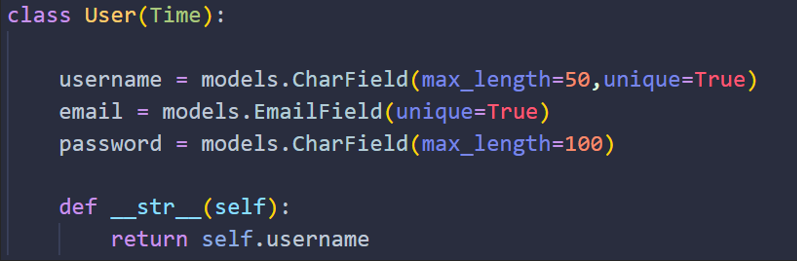
\includegraphics[width=\linewidth]{img/model.png}
    \caption{UserModel}
    \label{fig:etiqueta}
\end{figure}
\begin{itemize}
    \item Tabla \texttt{User} atributos: \texttt{username}, \texttt{email} y \texttt{password}
\end{itemize}

Se realizaron serializers para trabajar con las API que sirven para instanciar modelos.

\begin{figure}[htbp]
    \centering
    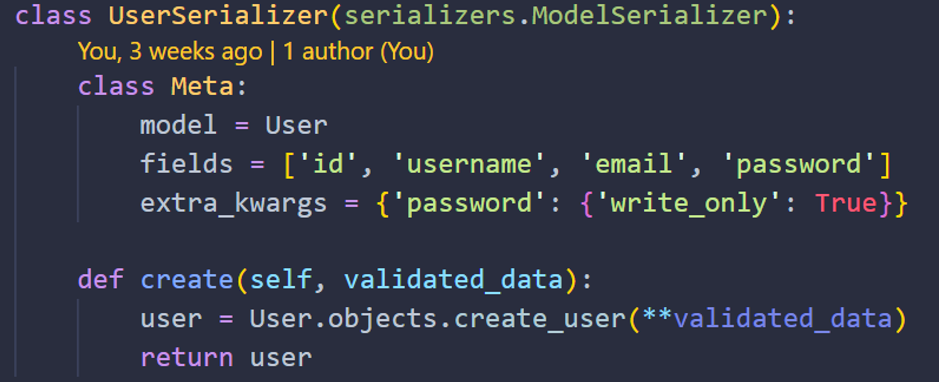
\includegraphics[width=\linewidth]{img/serializers.png}
    \caption{UserSerializers}
    \label{fig:etiqueta}
\end{figure}


Agregamos las rutas \texttt{urls.py} para los endpoints, todos estos pasos se realizaron para manejar la lógica del proyecto. Agregamos archivos estáticos y configuramos \texttt{settings.py} para que pueda utilizarlos.

\begin{figure}[htbp]
    \centering
    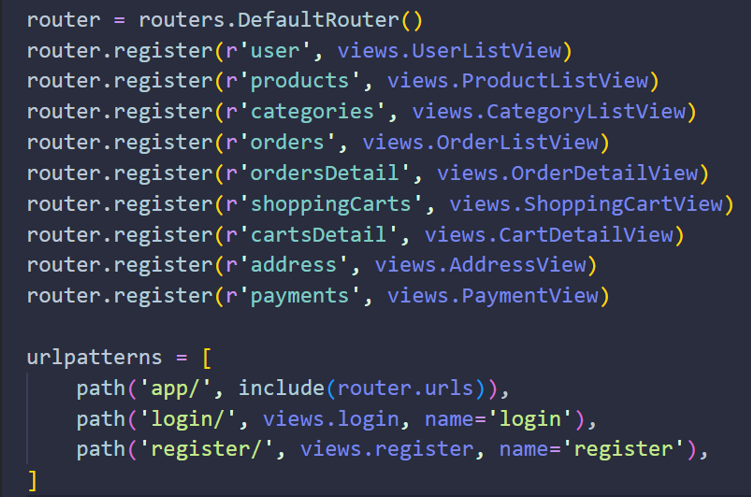
\includegraphics[width=\linewidth]{img/url.png}
    \caption{Urls}
    \label{fig:etiqueta}
\end{figure}

\subsection{Desarrollo del Frontend}
Para la realización del frontend se usó React para una mayor manejabilidad. Además de esto, se utilizó componentes esenciales como \texttt{ProductList} y \texttt{CreateProduct}.

\begin{verbatim}
import React, { useEffect, useState } from 'react';

const ProductList = () => {
  const [products, setProducts] = useState([]);
  const [loading, setLoading] = useState(true);
  const [error, setError] = useState(null);

  useEffect(() => {
    fetch('/api/products/')
      .then(response => {
        if (!response.ok) {
          throw new Error('Network response was not ok');
        }
        return response.json();
      })
      .then(data => {
        setProducts(data);
        setLoading(false);
      })
      .catch(error => {
        console.error('There was a problem with the fetch operation:', error);
        setError(error);
        setLoading(false);
      });
  }, []);

  if (loading) return <div>Loading...</div>;
  if (error) return <div>Error: {error.message}</div>;

  return (
    <div>
      <h1>Product List</h1>
      <ul>
        {products.map(product => (
          <li key={product.id}>{product.name} - ${product.price}</li>
        ))}
      </ul>
    </div>
  );
};

export default ProductList;
\end{verbatim}

Luego, hacemos uso del comando \texttt{npm run build}. Esto nos crea una carpeta \texttt{build}. Se trató de utilizar React Router para la navegación.

\subsection{Integración y Despliegue}
Para el despliegue en Heroku se usaron archivos estáticos, además de \texttt{whitenoise} y \texttt{gunicorn}. Además, se creó un archivo \texttt{Procfile}, que es lo que Heroku va a leer, por lo que es importante tenerlo en el archivo. Debe ir esto:

\begin{verbatim}
web: gunicorn tienda_online.wsgi --log-file -
\end{verbatim}

\begin{figure}[htbp]
    \centering
    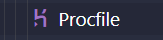
\includegraphics[width=\linewidth]{img/procfile.png}
    \caption{Procfile}
    \label{fig:etiqueta}
\end{figure}

Adicionalmente, se tuvo que crear una cuenta en Heroku para el uso. Posteriormente, Heroku te guía cómo conectarse a su servicio, que puede ser a través de \texttt{git}.

\begin{figure}[htbp]
    \centering
    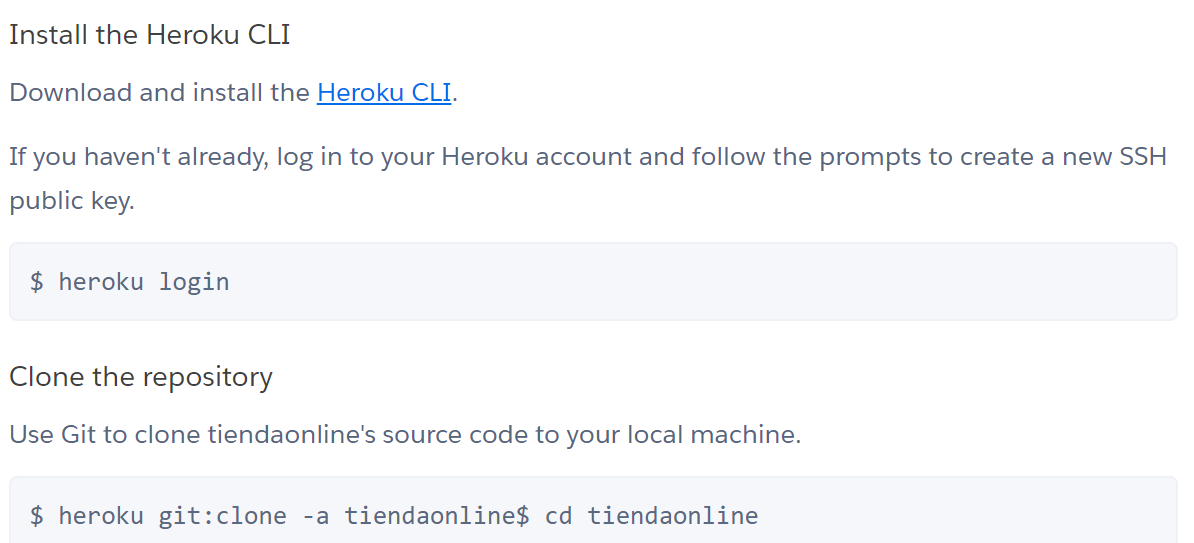
\includegraphics[width=\linewidth]{img/git.png}
    \caption{githeroku}
    \label{fig:etiqueta}
\end{figure}

Como observamos en la imagen, se indican los pasos para conectarse usando Heroku con comandos \texttt{git}. Una vez corriendo el proyecto, podemos colocar en la consola \texttt{heroku open} y automáticamente se abrirá la aplicación en nuestro navegador:

\url{https://tiendaonline-9c83954f4ca8.herokuapp.com/admin/}

\begin{figure}[htbp]
    \centering
    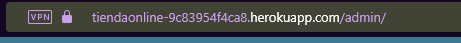
\includegraphics[width=\linewidth]{img/link.png}
    \caption{link}
    \label{fig:etiqueta}
\end{figure}

Podemos ver en django Admin (admin : 1234) como podemos ver nuestro datos y cambiarlos (agregando o eliminando) 

\begin{figure}[htbp]
    \centering
    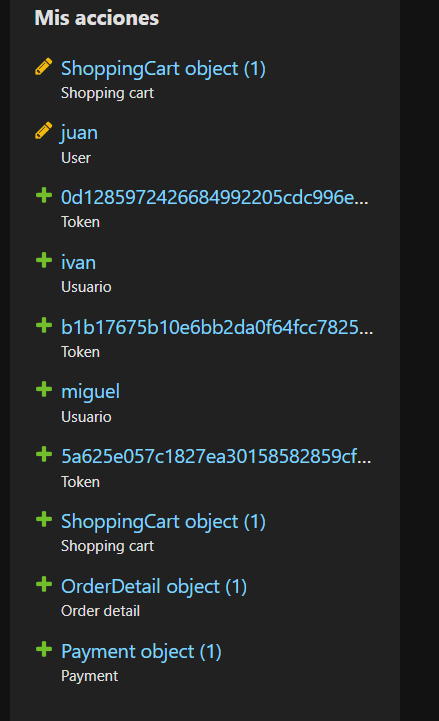
\includegraphics[width=\linewidth]{img/admin2.png}
    \caption{admin registros}
    \label{fig:etiqueta}
\end{figure}

\begin{figure}[htbp]
    \centering
    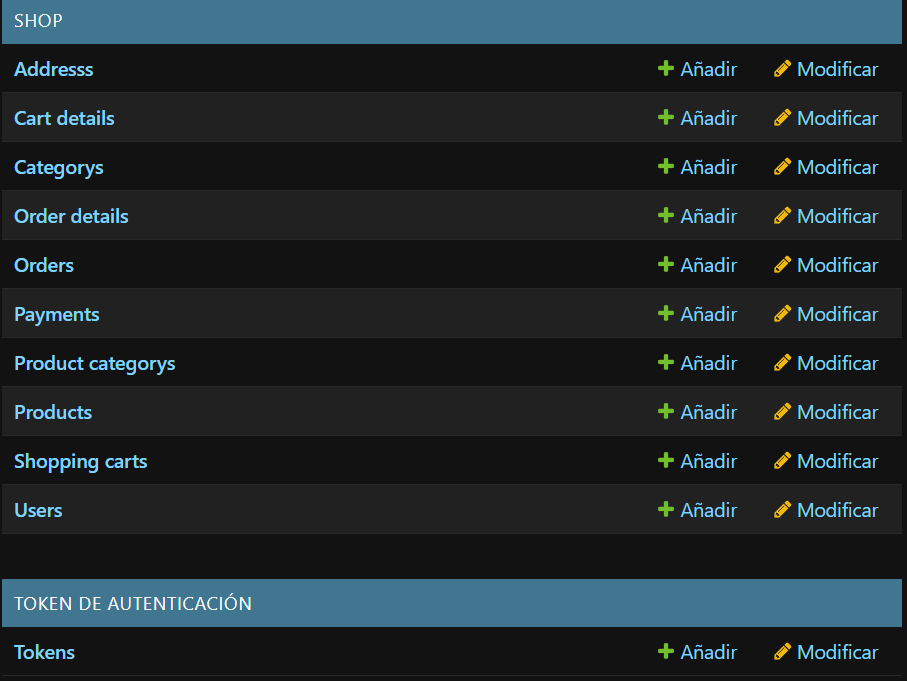
\includegraphics[width=\linewidth]{img/admin3.png}
    \caption{admin tablas}
    \label{fig:etiqueta}
\end{figure}
\section{Recomendaciones}
Este trabajo tiene mucho rango de mejora ya que no se exploró de manera muy profunda el desarrollo de estos. Pero satisfecho con el resultado propongo las siguientes mejoras:

\begin{itemize}
    \item \textbf{Escalabilidad}: Migrar a una base de datos más robusta como PostgreSQL o MySQL para manejar mayores volúmenes de datos.
    \item \textbf{Seguridad}: Implementar autenticación y autorización para proteger los datos y las operaciones del sistema.
    \item \textbf{Optimización de rendimiento}: Considerar el uso de técnicas como la compresión de imágenes y el uso de CDN para mejorar los tiempos de carga.
\end{itemize}

\section{Conclusiones}
El proyecto permitió explorar la integración de tecnologías frontend y backend, demostrando la eficacia de Django y React en la construcción de una aplicación. El despliegue en Heroku proporcionó una plataforma accesible, aunque se identificaron áreas para mejorar, especialmente en términos de seguridad y rendimiento. Así mismo, gracias a este trabajo, se pudo mejorar las habilidades con esta tecnología, solucionando problemas que se tuvieron al momento del desarrollo.

\begin{thebibliography}{9}
\bibitem{django} Tarantino, Q., Foxx, J., Waltz, C., \& DiCaprio, L. (2013). \textit{Django unchained}. Sony Pictures Home Entertainment.
\bibitem{react} Gackenheimer, C. (2015). \textit{Introduction to React}. Apress.
\bibitem{api_rest} Arsaute, A., Zorzán, F. A., Daniele, M., González, A., \& Frutos, M. (2018). Generación automática de API REST a partir de API Java basada en transformación de Modelos (MDD). In \textit{XX Workshop de Investigadores en Ciencias de la Computación (WICC 2018, Universidad Nacional del Nordeste)}.
\bibitem{sqlite} Owens, M., \& Allen, G. (2010). \textit{SQLite}. New York: Apress LP.
\bibitem{heroku} Lee, B. H., Dewi, E. K., \& Wajdi, M. F. (2018, April). Data security in cloud computing using AES under HEROKU cloud. In \textit{2018 27th wireless and optical communication conference (WOCC)} (pp. 1-5). IEEE.
\end{thebibliography}

\end{document}